% \documentclass[rnd]{mas_proposal}
\documentclass[thesis]{mas_proposal}

\usepackage[utf8]{inputenc}
\usepackage{amsmath}
\usepackage{amsfonts}
\usepackage{amssymb}
\usepackage{graphicx}
\usepackage{natbib} 

\title{Black-Box Optimization of Object Detector Hyper-Parameters}
\author{Mohandass Muthuraja}
\supervisors{Prof. Dr. Paul Pl̈oger \\ Dr. Matias Valdenegor-Toro}
\date{Month 20XX}

\thirdpartylogo{images/dfki.jpg}

\begin{document}

\maketitle

\pagestyle{plain}

\section{Introduction}
Object detection deals with classifying and localizing objects of interest in a given image or frame. In recent years, a great deal of research is done in object detection. It has various use cases such as autonomous cars, anomaly detection, medical image analysis, video surveillance and the list goes on. Recent advances in the deep learning architectures, mainly Convolutional Neural Networks (CNN) and the advent of parallel computing through Graphical Processing Units(GPU) has taken object detection a step forward. Deep learning-based object detection methods have proved to perform way better than traditional detection methods that use handcrafted features(such as SIFT\cite{lowe2004distinctive}, HoG\cite{dalal2005histograms}, etc.)\cite{zou2019object}. The ability of CNN architectures (such as VGG\cite{simonyan2014very}, Inception\cite{szegedy2015going}, DenseNet\cite{huang2017densely}, ResNet\cite{he2016deep} etc.,) to represent the high-level features of the image is one of the reasons for the remarkable performance of the state-of-the-art object detectors. These CNN architectures form the backbone of most state-of-the-art object detectors. Along with the CNN architectures, the region proposal network-based object detectors like Faster R-CNN\cite{ren2015faster}, R-FCN\cite{dai2016r} and  Mask R-CNN\cite{he2017mask} achieved extraordinary detection results. Moreover, object detectors like YOLO\cite{redmon2016you}, SSD\cite{liu2016ssd} and YOLOv2\cite{redmon2017yolo9000}  have proved to achieve remarkable results despite taking fewer computations\cite{zhao2019object}. 

% However, the performance of any deep learning algorithm depends heavily on the selection of various hyper-parameters that guide and controls the learning process. Each object detector has several hyper-parameters like image re-sizer dimensions, size and scales of prior/anchor boxes, Intersection Over Union (IOU) threshold, number of proposals in addition to the conventional deep learning hyper-parameters like learning rate, momentum and decay rate. The right choice of hyper-parameters here is essential as it plays a significant role in the model's performance. This task of hyper-parameter tuning is challenging as one need to choose the right hyper-parameter from the hyper-parameter search space efficiently. Machine learning experts and data scientists have intellectual depth and insight on setting hyper-parameters. Also, the experts conduct many experiments and choose hyper-parameters after many trial and errors. Besides, the hyper-parameters are dataset dependent as the hyper-parameters which works fine for one dataset may not perform better with another dataset\cite{automl_book}.
However, the performance of any deep learning algorithm depends heavily on the selection of various hyper-parameters that guide and controls the learning process. Each object detector has several hyper-parameters like image re-sizer dimensions, size and scales of prior/anchor boxes, Intersection Over Union (IOU) threshold, number of proposals in addition to the conventional deep learning hyper-parameters like learning rate, momentum and decay rate. This task of hyper-parameter tuning is challenging as one need to choose the right hyper-parameter from the hyper-parameter search space efficiently. Machine learning experts and data scientists have intellectual depth and insight on setting hyper-parameters. Besides, the hyper-parameters are dataset dependent as the hyper-parameters which works fine for one dataset may not perform better with another dataset\cite{automl_book}.

The tremendous growth of machine learning has created a need for automating this tedious process by avoiding human intervention. Automated machine learning (AutoML) is a newly emerging field which aims to automate the entire machine learning process. It includes automation of complete training pipeline right from data preprocessing, algorithm selection till setting the right hyper-parameters to obtain a obtain optimal performance\cite{automl_book}. Besides AutoML, black-box optimization methods can also be applied for the task of hyper-parameter optimization. Recent technical advancements in black-box optimization methods(such as Bayesian optimization, Genetic/Evolutionary algorithms) is getting more focused on hyper-parameter optimization. In this study, we will study AutoMl and black-box optimization methods for the task of setting hyper-parameters of object detectors on different datasets.
The main objectives of this study are as follows: 
\begin{itemize}
    \item A comprehensive literature study on the combined object detection and black-box optimization research fields.
    \item Defining the hyper-parameter search space of the state of the art deep convolutional object detectors.
    \item Comprehensive evaluation and comparison of  AutoMl and black-box optimization methods for hyper-parameter optimization specific to the state of the art object detectors on different datasets.
\end{itemize}
% \begin{itemize}
%     \item An introduction to the general topic you are covering.
%     \begin{itemize}
%     \item 3-4 sentences on object detection and CNNs in object detection
    
%     \item 3-4 sentences on importance of deep learning hyper parameters and object detection hyper parameters
%     \item 2-3 sentences on how experts decide the hyper parameters
%     \item 3-4 sentences on Auto Ml in the recent study
%     \item 3-4 general sentences on black box optimizer on deciding the hyper parameters
%     \item 3-4 sentences explaining what this project is about.
%     \end{itemize}
%     \item Why is it important?
    
% \end{itemize}

\subsection{Problem Statement}
% In the last decade, there was a breakthrough in one of the most challenging computer vision task of object detection. Classical object detectors that use handcrafted features are not able to meet the performance of the deep learning-based modern-day object detectors\cite{zou2019object}. The state of the art object detectors were able to achieve excellent performance on the MS-COCO\cite{lin2014microsoft} and PASCAL VOC\cite{Everingham10} benchmark datasets. The main challenge in achieving robust performance using these object detectors is the setting of hyper-parameters as they are heavily dataset dependent and requires experts' knowledge. The right choice of hyper-parameter selection from the over-all hyper-parameter space undergoes a lot of trial and error after conducting several experiments. Also, the diversity of the hyper-parameters turns out to be even more problematic in the task of hyper-parameter optimization because they can be binary, categorical(e.g. activation function), continuous(e.g. learning rates, drop-out probability),  and conditional(e.g. Adam's second momentum is active only when the optimizer is Adam)\cite{automl_book}.  The hyper-parameter space of the deep learning-based object detectors is also many in numbers as every object detector has its own hyper-parameters like re-sizer dimensions, size and scales of prior/anchor boxes, Intersection Over Union (IOU) threshold, number of proposals etc., The approach to solve this problem involves the use of hyper-parameter optimization methods after defining the hyper-parameter space of the object detectors. Most basic hyper-parameter optimization methods use grid search\cite{montgomery2001design} and random search\cite{bergstra2012random} to select the set of hyper-parameters to obtain better performance. However, both these searches take a considerable amount of time and are computationally expensive. A guided search can reduce the computational complexity and time taken to find the right set of parameters.  
 The state of the art object detectors were able to achieve excellent performance on the MS-COCO\cite{lin2014microsoft} and PASCAL VOC\cite{Everingham10} benchmark datasets. Classical object detectors that use handcrafted features are not able to meet the performance of the deep learning-based modern-day object detectors\cite{zou2019object}. The main challenge in achieving robust performance using the deep learning-based object detectors is the setting of hyper-parameters as they are heavily dataset dependent and requires experts' knowledge. The right choice of hyper-parameter selection from the over-all hyper-parameter space undergoes a lot of trial and error after conducting several experiments. Also, the diversity of the hyper-parameters turns out to be even more problematic in the task of hyper-parameter optimization because they can be binary, categorical(e.g. activation function), continuous(e.g. learning rates, drop-out probability),  and conditional(e.g. Adam's second momentum is active only when the optimizer is Adam)\cite{automl_book}.  The hyper-parameter space of the deep learning-based object detectors is also many in numbers as every object detector has its own hyper-parameters like re-sizer dimensions, size and scales of prior/anchor boxes, Intersection Over Union (IOU) threshold, number of proposals etc., The approach to solve this problem involves the use of hyper-parameter optimization methods after defining the hyper-parameter space of the object detectors. Most basic hyper-parameter optimization methods use grid search\cite{montgomery2001design} and random search\cite{bergstra2012random} to select the set of hyper-parameters to obtain better performance. However, both these searches take a considerable amount of time and are computationally expensive. A guided search can reduce the computational complexity and time taken to find the right set of parameters. 
AutoML and Black-box optimization techniques have been applied to image classification successfully for neural architecture search and hyper-parameter optimization. Using AutoML and Black-box optimization techniques for object detection is a new open research topic which is gaining more importance among the researchers in the computer vision community. This proposed research work intends to study the applicability of the modern hyper-parameter optimization methods of AutoML and Black-box optimization. These methods will be used to tune the hyper-parameter particular to the deep-learning-based state of the art object detectors to achieve the optimal performance.  The hyper-parameter optimization task will be evaluated on a variety of datasets. Also, the idea is to guide the tuning process to balance the trade-off between high object detection performance and fewer computations.
% \begin{itemize}
%     \item What are you going to solve?
%     \begin{itemize}
%         \item Problems with random and grid search, Computational complexity , deciding the hyper parameters
%         \item How this can be solved using BBO
%     \end{itemize}
%     \item How are you evaluating?
% \end{itemize}


\section{Related Work}
% \begin{itemize}
%     \item What have other people done?
%     \begin{itemize}
%         \item Literature on SOTA object detection models
        
%         \item Literature on BBO techniques
%     \end{itemize}
%     \item Why is it not sufficient?
% \end{itemize}

\subsection{Object Detection}
Deep learning-based object detectors can be grouped into two types, namely, multi-stage detectors and single-stage detectors. Multi-stage detectors initially involve the selection of regions of interest(ROI) from an image and then detecting the class on those regions. In spite of obtaining remarkable results, multi-stage detectors need more computations. Single-stage detectors are faster than the multi-stage detectors as it does a combined task of locating and then classifying the objects in the image. 

\subsubsection{Multi-stage Detectors}

\textbf{R-CNN} by \citet{girshick2014rich} provided a breakthrough in 2014 by achieving 30\% better performance on the Pascal-VOC 2012 dataset. RCNN has three main steps. First, selective search algorithm was used to generate around 2000 regions on the image. Next, CNN's were used to extract a 4096-dimensional feature vector from those regions. Finally, the extracted features were classified using SVMs. 

\textbf{Fast R-CNN} by \citet{girshick2015fast} sorted out the issues in R-CNN by an alternative approach. First, instead of region proposals, the entire image was fed into CNN's to get a convolutional feature map. Then, the region proposals were determined on the convolutional feature map. Finally, the region proposals that were reshaped by ROI pooling layer were fed into a fully connected layer for classifying the objects. Fast R-CNN is faster because the convolution operation is done only once on the entire image instead of 2000 regions as in the case of R-CNN. 

\textbf{Faster R-CNN} by \citet{ren2015faster} introduced a Region Proposal Network(RPN) for identifying the region proposals which replaced the selective search algorithm in R-CNN and Fast R-CNN. The use of RPN instead of selective search algorithm proves to be more time-efficient and also has a better performance. In, Faster R-CNN, first, the image is fed into CNN's to produce a  convolutional feature map. Then the RPN provides region proposal from the convolutional feature map. Same like Fast R-CNN, these region proposals were reshaped by ROI pooling layer were fed into a fully connected layer for classifying the objects.

\subsubsection{Single stage Detectors}
\citet{redmon2016you} introduced a fast and accurate object detector called \textbf{YOLO}(You Look Only Once). Unlike the other multi-stage object detectors, YOLO considers object detection as a regression problem to determine the bounding box coordinates of the objects in the image and their corresponding class probabilities. YOLO uses a single neural network to perform the complete object detection. First, YOLO transforms the image into a grid of specific size. Then, in each grid, it considers bounding boxes and the network is trained to determine the bounding box offsets and the class probabilities. YOLO finds its use in applications which involve real-time predictions as it can predict 45 frames per second. The inadequacy of YOLO is that it is not good with smaller objects. To improve the accuracy and to balance the speed-accuracy trade-off, further improvements were made on its successive version YOLO v2 \cite{redmon2017yolo9000}. 

Single ShotMultiBox Detector (\textbf{SSD})  proposed by \citet{liu2016ssd} is another single stage object detector. SSD can overcome the deficit of YOLO as it performs well with smaller objects also. The vital feature of SSD is the multi-scale convolutional bounding box. Instead of the fixed grids in YOLO, SSD initially 'discretizes the output space of bounding boxes into a set of default boxes over different aspect ratios and scales per feature map location.'\cite{liu2016ssd} Despite being three times faster, SSD512 model performs better than faster R-CNN on PASCAL VOC and COCO datasets. 

\textbf{RetinaNet} proposed by \citet{lin2017focal} addresses the foreground-background class imbalance issue in the previous object detectors. RetinaNet has a particular loss function called 'focal loss' loss function. This helps the single-stage detectors to achieve competitive results with the multi-stage detectors by not compromising the speed.  

\subsection{Black-box Hyper parameter Optimization}

% \textbf{Grid search}\cite{montgomery2001design} is the primitive and conventional method used for hyper parameter optimization. It is a brute force search algorithm which enumerates all possible set of hyper-parameters from the hyper-parameter space. However, because of the potential increase of the function evaluations with the rise in the number of hyper-parameters, it suffers from an aspect called "curse of dimensionality"\cite{friedman2018recursive}.

% \textbf{Random search}\cite{bergstra2012random} samples the hyper-parameter from the defined hyper-parameter space and evaluates those samples. In this way, it reduces the number of evaluation, but it doesn't consider the results from the previous evaluation to sample the next set of hyper-parameters. Due to this, it takes more longer than any guided search algorithm to find the best set of hyper-parameters.  

\textbf{Bayesian optimization}\cite{movckus1975bayesian} is a guided way to find the best combination of hyper-parameters as it considers prior information. Bayesian optimization is used in finding the set of hyper-parameters in various deep learning networks. It has proved to achieve better results with fewer computations when compared to the grid and random search in image classification, speech recognition and natural language modelling \cite{snoek2012practical}\cite{snoek2015scalable}\cite{melis2017state}\cite{dahl2013improving}. In Bayesian optimization, initially a random set of hyper-parameters are evaluated, and then a probabilistic model is fit to this data in the hyper-parameter space. Then, the model is used by a function called acquisition function to determine the next sampling point(set of hyper-parameters) that has to be evaluated. This process goes in iteration until a computational budget is met. The shortcoming of the Bayesian optimization is that it is not robust when the hyper-parameter space is complex and conditional \cite{wang2013bayesian} \cite{swersky2014raiders}.
Bayesian optimization using Tree Parzen Estimator(TPE) can handle categorical hyper-parameters and can work in parallel.\cite{bergstra2011algorithms}.\cite{feurer_hyperparameter_2018}  

\textbf{Hyperband }by \citet{li2016hyperband} is a reinforcement-based learning approach for hyper-parameter optimization which considers HPO as a non-stochastic infinite-armed bandit problem. Hyperband shows better results than the bayesian optimization that doesn't count low fidelities.\cite{li2016hyperband}\cite{feurer_hyperparameter_2018}

\textbf{Bayesian Optimization and Hyperband} (BOHB) by \citet{falkner2018bohb}  is a combined algorithm of Bayesian optimization(with TPE) and hyperband for HPO.  BOHB is very easy to implement, robust and adaptable for various type of hyper-parameters.  It performs better than the Bayesian optimization and hyperband on a variety of problems and benchmarks. \cite{falkner2018bohb}\cite{feurer_hyperparameter_2018}

\textbf{Population-based} approaches, namely Genetic Algorithm(GA), Genetic Programming(GP), Evolutionary strategy(ES), Evolutionary Programming(EP) and Particle Swarm Optimization have shown remarkable results in optimization problems\cite{coello2007evolutionary}. The most significant advantage of the population-based approach is the evaluations of hyper-parameters can run in parallel.  Co-variance Matrix Adaptation Evolution Strategy (CMA-ES) is a successful population-based approach for hyper-parameter optimization\cite{loshchilov2016cma} and also one of the best performing algorithms for hyper-parameter optimization in the Black-Box Optimization Benchmarking(BBOB) challenge\cite{bbob}. \citet{loshchilov2016cma} has applied CMA-ES for hyper-parameter optimization of convolutional neural network(CNN) for MNIST data classification problem and has parallelly used 30 GPU's.  Particle Swarm Optimization algorithm is also proved beneficial for a hyper-parameter optimization problem. \citet{lorenzo2017particle} has applied Particle Swarm Optimization(PSO) for optimizing the Deep Neural Net(DNN) classifier on the CIFAR-10 dataset. \citet{lorenzo2017hyper} used the PSO to perform the hyper-parameter optimization parallelly and quickly. \cite{feurer_hyperparameter_2018}

The above mentioned hyper-parameter optimization methods have been used in various machine learning algorithms and Deep Neural Networks(DNN's) for tuning the hyper-parameters. AutoML and black-box optimization methods have been successful in deep-learning-based image classification successfully for neural architecture search and hyper-parameter optimization. However, these methods have not been explored much in tuning the Deep learning-based object detectors. In this thesis work, automatic tuning of hyper-parameters for the deep-learning-based object detectors will be studied. 

\section{Project Plan}

% \subsection{Work Packages}
% The bare minimum will include the following packages:
% \begin{enumerate}
%     \item[WP1] Literature Search
%     \item[WP2] Experiments
%     \item[WP3] Project Report
% \end{enumerate}
% Keep in mind that depending on your project, you will probably need to add work packages that are more suited to your projects.

\subsection{Milestones}
\begin{enumerate}
    \item[M1] Literature search and state of the art analysis
    \item[M2] Defining Object detector parameter space and training pipeline setup
    \item[M3] Hyper-parameter optimization pipeline setup 
    \item[M4] Complete experimental design for HPO on object detectors
    \item[M5] Experimental trials and Analysis
    \item[M6] Initial report draft 
    \item[M7] Report submission
\end{enumerate}
\newpage
\subsection{Project Schedule}
% \begin{figure}[h!]
%     \caption{}
%     \includegraphics[width=\textwidth]{images/rnd_deliverable_timeline}
%     \label{}
% \end{figure}
\begin{figure}[!htb]
    \caption{Gannt Chart for project timeline}
    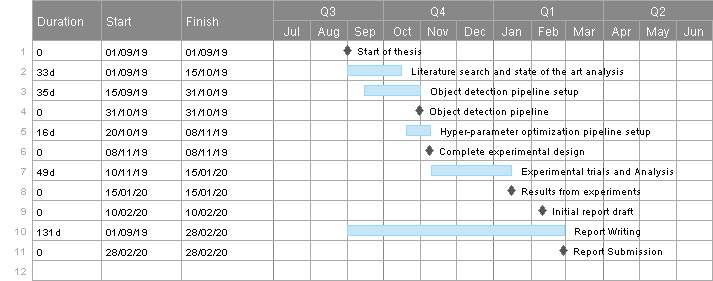
\includegraphics[width=\textwidth]{images/ThesisProposal.png}
    \label{Thesis_Timeline}
\end{figure}
\subsection{Deliverables}
\subsubsection*{Minimum Viable}

% \begin{itemize}
%     \item Survey
%     \item Analysis of state of the art
%     \item Simple simulated use case
%     \item Demo on youBot or Jenny
% \end{itemize}
\begin{itemize}
    \item Literature search and state of the art analysis on the  combined object detection and black-box optimization  fields.

\end{itemize}

\subsubsection*{Expected}
\begin{itemize}
    \item Appropriate experimental design to address the hyper-parameter optimization for object detectors.
    \item Comprehensive evaluation and comparison with the state of the art on the datasets like COCO and PASCAL VOC on at least two object detectors.
\end{itemize}

\subsubsection*{Desired}
\begin{itemize}
    \item  Conference or journal paper describing the results from the Thesis
\end{itemize}


\nocite{*}

\bibliographystyle{plainnat} % Use the plainnat bibliography style
\bibliography{bibliography.bib} % Use the bibliography.bib file as the source of references




\end{document}
